\section{Introduction}

Generative modeling is a core problem in machine learning, useful both for benchmarking our ability to capture statistics of natural datasets and for downstream applications that require generating high-dimensional data like images, text, and speech waveforms.
There has been a great deal of progress with the development of methods like GANs~\citep{goodfellow2014generative,brock2018large}, VAEs~\citep{kingma2013auto,rezende2014stochastic}, large autoregressive neural network models~\citep{oord2016pixel,oord2016wavenet,vaswani2017attention}, normalizing flows~\citep{rezende2015variational, dinh2016density, kingma2018glow,papamakarios2019normalizing}, and others, each with their own tradeoffs in terms of sample quality, sampling speed, log-likelihoods, and training stability.

Recently, diffusion models \citep{sohl2015deep} have emerged as a compelling alternative for  image~\citep{ho2020denoising,song2020improved} and audio~\citep{wavegrad,kong2020diffwave} generation, achieving comparable sample quality to GANs and log-likelihoods comparable to autoregressive models with fewer inference steps. 
A diffusion model is a parameterized Markov chain trained to reverse a predefined forward process, which is a stochastic process constructed to gradually corrupt training data into pure noise.
Diffusion models are trained using a stable objective closely related to both maximum likelihood and score matching~\citep{hyvarinen2004independent,vincent2011connection}, and they admit faster sampling than autoregressive models by using parallel iterative refinement~\citep{nichol2021improved,song_2019,song2020_sde,song2021implicit}.

Although diffusion models have been proposed in both discrete and continuous state spaces~\citep{sohl2015deep}, most recent work has focused on Gaussian diffusion processes that operate in continuous state spaces (e.g. for real-valued image and waveform data). Diffusion models with discrete state spaces have been explored for text and image segmentation domains \citep{hoogeboom2021argmax}, but they have not yet been demonstrated as a competitive model class for large scale text or image generation.


\begin{figure}
    \centering
    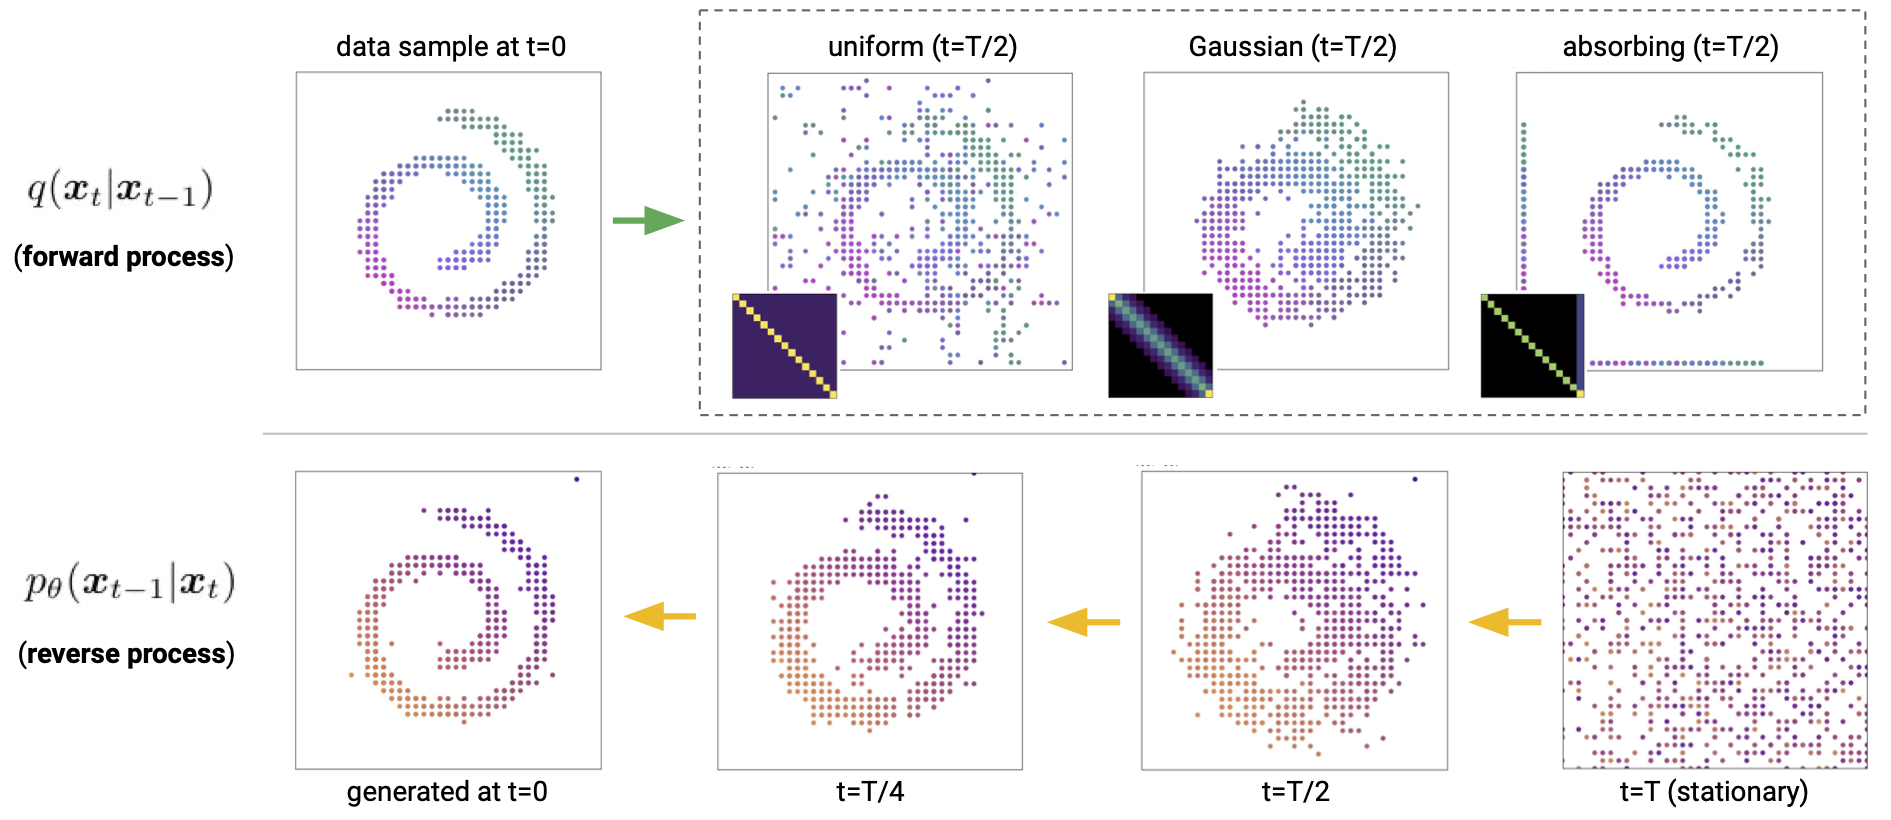
\includegraphics[width=0.95\textwidth]{figures/final.png}
    \caption{D3PM forward and (learned) reverse process applied to a quantized swiss roll. Each dot represents a 2D categorical variable. Top: samples from the uniform, discretized Gaussian, and absorbing state D3PM model forward processes, along with corresponding transition matrices $\bQ$. Bottom: samples from a learned discretized Gaussian reverse process.}
    \label{fig:swiss_roll}
    \vspace{-0.3cm}
\end{figure}
Our aim in this work is to improve and extend discrete diffusion models by using a more structured categorical corruption process to shape data generation, as illustrated in Figure~\ref{fig:swiss_roll}. Our models do not require relaxing or embedding discrete data (including images) into continuous spaces, and can embed structure or domain knowledge into the transition matrices used by the forward process. We achieve significantly improved results by taking advantage of this flexibility. We develop structured corruption processes appropriate for text data, using similarity between tokens to enable gradual corruption and denoising. Expanding further, we also explore corruption processes that insert [MASK] tokens, which let us draw parallels to autoregressive and mask-based generative models. Finally, we study discrete diffusion models for quantized images, taking inspiration from the locality exploited by continuous diffusion models. This leads to a particular choice of discrete corruption process that diffuses preferentially to more similar states and leads to much better results in the image domain. 

Overall, we make a number of technical and conceptual contributions.
Beyond designing several new structured diffusion models, we introduce a new auxiliary loss which stabilizes training of D3PMs and a family of noise schedules based on mutual information that lead to improved performance. We strongly outperform various non-autoregressive baselines for text generation on character-level text generation, and successfully scale discrete diffusion models to large vocabularies and long sequence lengths. We also achieve strong results on the image dataset CIFAR-10, approaching or exceeding the Gaussian diffusion model from \citet{ho2020denoising} on log-likelihoods and sample quality. 


